% Team 20 (P20) project report, Natural Language Engineering (nle) template from the course.
% Compile on Overleaf inside the template project that ships nle.cls.
% Every \TBD{} is a number still to be filled from results/tables.md (python -m src.make_tables).
% Never replace a \TBD{} with a number that is not in results/*/*/metrics.json.

\documentclass{nle}

\usepackage{graphicx}
\newcommand\TBD[1]{\textbf{[#1]}}
\newcommand\eg{{\it e.g.\ }}

\title[Detecting AI-Generated Text Across Domains and Generators]
      {Detecting AI-Generated Text Across Domains and Generators:\\
       Generalisation to Unseen Generators, Domains and Paraphrases}
\author[N.\ Kumar and others]
       {N\ls I\ls R\ls M\ls A\ls L\ns K\ls U\ls M\ls A\ls R,\ns
        V\ls I\ls V\ls E\ls K\ns K\ls U\ls M\ls A\ls R,\ns
        R\ls I\ls T\ls E\ls S\ls H\ns J\ls H\ls A\ns
        and\ns V\ls I\ls S\ls H\ls A\ls L\ns K\ls U\ls M\ls A\ls R\\
        Team 20, Deep Learning course, Sitare}

\received{22 November 2026}
\pagerange{\pageref{firstpage}--\pageref{lastpage}}
\pubyear{2026}

\begin{document}

\label{firstpage}
\maketitle

\begin{abstract}
Detectors of machine-generated text are usually evaluated on the same generators and domains they were trained on.
We study how well they generalise. Using the English part of the M4 benchmark (5 domains $\times$ 5 generators,
38,241 texts after cleaning), we compare a TF-IDF + logistic regression baseline, a fine-tuned RoBERTa classifier and
three zero-shot scores computed with GPT-2 medium (mean log-likelihood, log-rank and Fast-DetectGPT). Every detector is
evaluated in four settings: in-distribution, leave-one-generator-out, leave-one-domain-out, and a paraphrase attack
in which the same 500 machine texts are rewritten by a T5 paraphraser. Splits are made by group so that no human text,
or machine text written for the same prompt, appears in both training and test, and all methods are graded by one
shared evaluator (AUROC with group-bootstrap 95\% confidence intervals, accuracy and macro-F1 at a validation-chosen
threshold, and TPR at 1\% FPR). \TBD{One or two sentences with the main findings, from Tables 1--4.}
\end{abstract}

\section{Introduction}

Large language models (LLMs) now write fluent text in every domain, which creates a need to tell human-written text
from machine-generated text, for example in education and content moderation. Detectors fall into two families:
supervised classifiers trained on labelled examples, and zero-shot methods that score a text with a language model
without any training \cite{mitchell23}. A supervised detector can reach very high accuracy on the generators it was
trained on, but in practice a detector meets text from new generators, new domains, and text that was deliberately
rewritten to evade it.

The project brief (P20) asks us to distinguish human-written from LLM-generated text and to test generalisation to
unseen generators, using M4 \cite{wang24}, with a TF-IDF + LR baseline, a fine-tuned RoBERTa detector, zero-shot
perplexity / DetectGPT-style scoring and leave-one-generator-out evaluation, and to report cross-generator and
cross-domain robustness and the effect of paraphrasing attacks. Our contributions are:
\begin{itemize}
  \item a cleaned, group-aware version of M4 English with 12 evaluation settings (in-distribution, 5 held-out
        generators, 5 held-out domains, and a paraphrase before/after pair), released as split files;
  \item one shared evaluator so that every method is graded the same way, with guards against leakage;
  \item a comparison of five detectors across all settings, plus a length-only shortcut check;
  \item a paraphrase attack that keeps the human texts fixed, so the change in AUROC is caused by the paraphrase alone.
\end{itemize}

\section{Related work}

M4 \cite{wang24} is a multi-generator, multi-domain and multi-lingual benchmark for machine-generated text detection.
Its authors show that detectors trained on some generators or domains degrade on others, which motivates our
leave-one-out settings. DetectGPT \cite{mitchell23} observes that machine text tends to lie near a local maximum of
the model's log-probability and measures this \emph{probability curvature} by comparing the log-probability of a text
with that of perturbed copies. Fast-DetectGPT \cite{bao24} replaces the perturbations by an analytic estimate of the
same quantity computed from a single forward pass. Fine-tuned RoBERTa classifiers \cite{liu19} are a strong
supervised baseline for this task.

\section{Data}

\subsection{Source and sampling}
We use the English part of M4: human texts paired with texts generated for the same prompt by ChatGPT, davinci-003,
Cohere, Dolly-v2 and BLOOMZ, in Wikipedia, wikiHow, Reddit ELI5, arXiv abstracts and PeerRead reviews. The full
$5 \times 5$ grid exists; files that exist only for some domains (FLAN-T5, LLaMA) are left out so that every setting
covers the same generators. We keep at most 1,000 pairs per (domain, generator) cell (PeerRead: 250 papers per cell,
about four machine reviews each), drop texts under 50 characters and machine texts that copy the prompt, and use seed
42 throughout. The final dataset has 38,241 texts: 13,243 human and 24,998 machine, in 11,278 groups.

\subsection{Cleaning}
Three choices matter for a fair evaluation. (i) \emph{Whitespace is collapsed in every text}: arXiv and PeerRead human
texts contain hard line breaks that machine texts do not, which a detector could exploit as a formatting shortcut.
(ii) For BLOOMZ we take the output-only field, because its \texttt{machine\_text} field contains the prompt.
(iii) The same human text appears in up to five generator files; we keep it once and give it, and all its machine
twins, the same \emph{group} identifier (a hash of the human text; for PeerRead, of the paper).

\subsection{Evaluation settings and group-aware splits}
Splits are made by group, never by row, so no human text and no machine text written for the same prompt appears on
both sides of a split. Table~\ref{tab:settings} lists the settings.

\begin{table}
  \caption{Evaluation settings. All splits are by group. Sizes from \texttt{results/data\_audit.md}.}
  \begin{tabular}{llll}
  \hline\hline
  Setting & Train / val & Test & Question \\
  \hline
  \texttt{indist} & 80\% / 10\% of groups & other 10\% & same generators and domains \\
  \texttt{logo\_<gen>} ($\times$5) & other 4 generators & only \texttt{<gen>} & unseen generator \\
  \texttt{xdomain\_<dom>} ($\times$5) & other 4 domains & only \texttt{<dom>} & unseen domain \\
  \texttt{paraphrase\_orig} $\to$ \texttt{paraphrase} & \texttt{indist} model & 500 machine + 500 human & paraphrase attack \\
  \hline\hline
  \end{tabular}
  \label{tab:settings}
\end{table}

\texttt{indist} has 30,602 / 3,801 / 3,838 texts; each LOGO test set has about 10,100 texts and each cross-domain
test set about 7,500. In a LOGO setting, the test groups keep only their human texts and the held-out generator's
texts; the other generators' texts in those groups are dropped rather than moved to training, so no test human text is
seen during training. Because each human text is kept once, machine texts outnumber human texts (about 1.9 : 1 in
\texttt{indist}); trained models use class weights, and AUROC does not depend on the ratio.

\section{Methods}

Every detector outputs one score per text, with higher meaning more likely machine-generated.

\paragraph{Length-only baseline.} Logistic regression on log(characters) and log(words). It is not a real detector
but a shortcut check: where it scores well, part of every detector's score may come from text length.

\paragraph{TF-IDF + logistic regression.} Word 1--2-grams (up to 200k features) and character 3--5-grams (up to 300k
features) with sublinear TF, concatenated, then logistic regression with balanced class weights. The regularisation
strength $C \in \{0.25, 1, 4, 16\}$ is selected by validation AUROC in each setting.

\paragraph{Fine-tuned RoBERTa.} \texttt{roberta-base} with a two-class head, inputs truncated to 256 tokens, one epoch,
batch size 16, learning rate $2\cdot10^{-5}$ with AdamW, 6\% warm-up and linear decay, fp16 on a T4 GPU, and
class-weighted cross-entropy. Validation AUROC is computed twice per epoch and the best checkpoint is kept.

\paragraph{Zero-shot scores.} GPT-2 medium scores each text truncated to 256 tokens.
\emph{Log-likelihood} (\texttt{ppl}) is the mean token log-probability; \emph{log-rank} is minus the mean log-rank of
the actual tokens; \emph{Fast-DetectGPT} \cite{bao24} is
\[
  \frac{\sum_t \log p(x_t) - \sum_t \mu_t}{\sqrt{\sum_t \sigma_t^2}},
\]
where $\mu_t$ and $\sigma_t^2$ are the mean and variance of $\log p$ under the model's own next-token distribution at
position $t$. Because of the compute budget, Fast-DetectGPT scores a fixed subset of 1,500 texts (the 1,000
\texttt{paraphrase\_orig} test texts plus 500 balanced validation texts) together with the paraphrase test sets.

\paragraph{Paraphrase attack.} The 500 machine texts of the \texttt{paraphrase\_orig} test set are paraphrased sentence
by sentence with a T5 paraphraser (\texttt{humarin/chatgpt\_paraphraser\_on\_T5\_base}, nucleus sampling $p=0.9$,
temperature 0.8); sentences longer than 60 words are split first so the input is never truncated. The
\texttt{paraphrase} setting uses the same humans with the machine texts replaced, and every detector uses its
\texttt{indist} model without retraining. As a control, 200 human texts are paraphrased as well
(\texttt{paraphrase\_human}, label still human).

\section{Evaluation protocol}

All methods write predictions in one format and are graded by one script. True labels come from the dataset, never
from the detector, and the evaluator rejects any prediction file that scores a training text, misses a test text (only
Fast-DetectGPT may score a subset), or contains duplicate or non-finite scores. We report AUROC on the test set with a
95\% confidence interval from 1,000 bootstrap resamples of whole groups (texts in a group are not independent);
accuracy and macro-F1 at the threshold that maximises macro-F1 on the \emph{validation} set, applied unchanged to
test (omitted when validation has fewer than 50 texts per class); and the true positive rate at 1\% false positive
rate, reported only when the test set has at least 1,000 human texts.

\section{Results}

\TBD{Tables 1--4 and Figures 1--2 are generated by \texttt{python -m src.make\_tables} into
\texttt{results/tables.md} and \texttt{results/figures/}. Copy the numbers here; settings that could not be run are
written as ``not run (compute)''.}

\begin{table}
  \caption{In-distribution test results (\texttt{indist}).}
  \begin{tabular}{lcccc}
  \hline\hline
  Method & AUROC [95\% CI] & Accuracy & Macro-F1 & TPR@1\%FPR \\
  \hline
  Length only     & \TBD{} & \TBD{} & \TBD{} & \TBD{} \\
  TF-IDF + LR     & \TBD{} & \TBD{} & \TBD{} & \TBD{} \\
  Log-likelihood  & \TBD{} & \TBD{} & \TBD{} & \TBD{} \\
  Log-rank        & \TBD{} & \TBD{} & \TBD{} & \TBD{} \\
  Fast-DetectGPT  & \TBD{} & \TBD{} & \TBD{} & \TBD{} \\
  RoBERTa         & \TBD{} & \TBD{} & \TBD{} & \TBD{} \\
  \hline\hline
  \end{tabular}
  \label{tab:indist}
\end{table}

\begin{table}
  \caption{Leave-one-generator-out AUROC (column = held-out generator).}
  \begin{tabular}{lcccccc}
  \hline\hline
  Method & ChatGPT & davinci & Cohere & Dolly & BLOOMZ & Mean \\
  \hline
  Length only     & \TBD{} & \TBD{} & \TBD{} & \TBD{} & \TBD{} & \TBD{} \\
  TF-IDF + LR     & \TBD{} & \TBD{} & \TBD{} & \TBD{} & \TBD{} & \TBD{} \\
  Log-likelihood  & \TBD{} & \TBD{} & \TBD{} & \TBD{} & \TBD{} & \TBD{} \\
  Log-rank        & \TBD{} & \TBD{} & \TBD{} & \TBD{} & \TBD{} & \TBD{} \\
  Fast-DetectGPT  & \TBD{} & \TBD{} & \TBD{} & \TBD{} & \TBD{} & \TBD{} \\
  RoBERTa         & \TBD{} & \TBD{} & \TBD{} & \TBD{} & \TBD{} & \TBD{} \\
  \hline\hline
  \end{tabular}
  \label{tab:logo}
\end{table}

\begin{table}
  \caption{Cross-domain AUROC (column = held-out domain).}
  \begin{tabular}{lcccccc}
  \hline\hline
  Method & Wikipedia & wikiHow & Reddit & arXiv & PeerRead & Mean \\
  \hline
  Length only     & \TBD{} & \TBD{} & \TBD{} & \TBD{} & \TBD{} & \TBD{} \\
  TF-IDF + LR     & \TBD{} & \TBD{} & \TBD{} & \TBD{} & \TBD{} & \TBD{} \\
  Log-likelihood  & \TBD{} & \TBD{} & \TBD{} & \TBD{} & \TBD{} & \TBD{} \\
  Log-rank        & \TBD{} & \TBD{} & \TBD{} & \TBD{} & \TBD{} & \TBD{} \\
  Fast-DetectGPT  & \TBD{} & \TBD{} & \TBD{} & \TBD{} & \TBD{} & \TBD{} \\
  RoBERTa         & \TBD{} & \TBD{} & \TBD{} & \TBD{} & \TBD{} & \TBD{} \\
  \hline\hline
  \end{tabular}
  \label{tab:xdomain}
\end{table}

\begin{table}
  \caption{Paraphrase attack: AUROC on the same 500 machine and 500 human texts before and after paraphrasing.}
  \begin{tabular}{lcccc}
  \hline\hline
  Method & Original & Paraphrased & Drop & Human-paraphrase control \\
  \hline
  Length only     & \TBD{} & \TBD{} & \TBD{} & \TBD{} \\
  TF-IDF + LR     & \TBD{} & \TBD{} & \TBD{} & \TBD{} \\
  Log-likelihood  & \TBD{} & \TBD{} & \TBD{} & \TBD{} \\
  Log-rank        & \TBD{} & \TBD{} & \TBD{} & \TBD{} \\
  Fast-DetectGPT  & \TBD{} & \TBD{} & \TBD{} & \TBD{} \\
  RoBERTa         & \TBD{} & \TBD{} & \TBD{} & \TBD{} \\
  \hline\hline
  \end{tabular}
  \label{tab:para}
\end{table}

% \begin{figure}
%   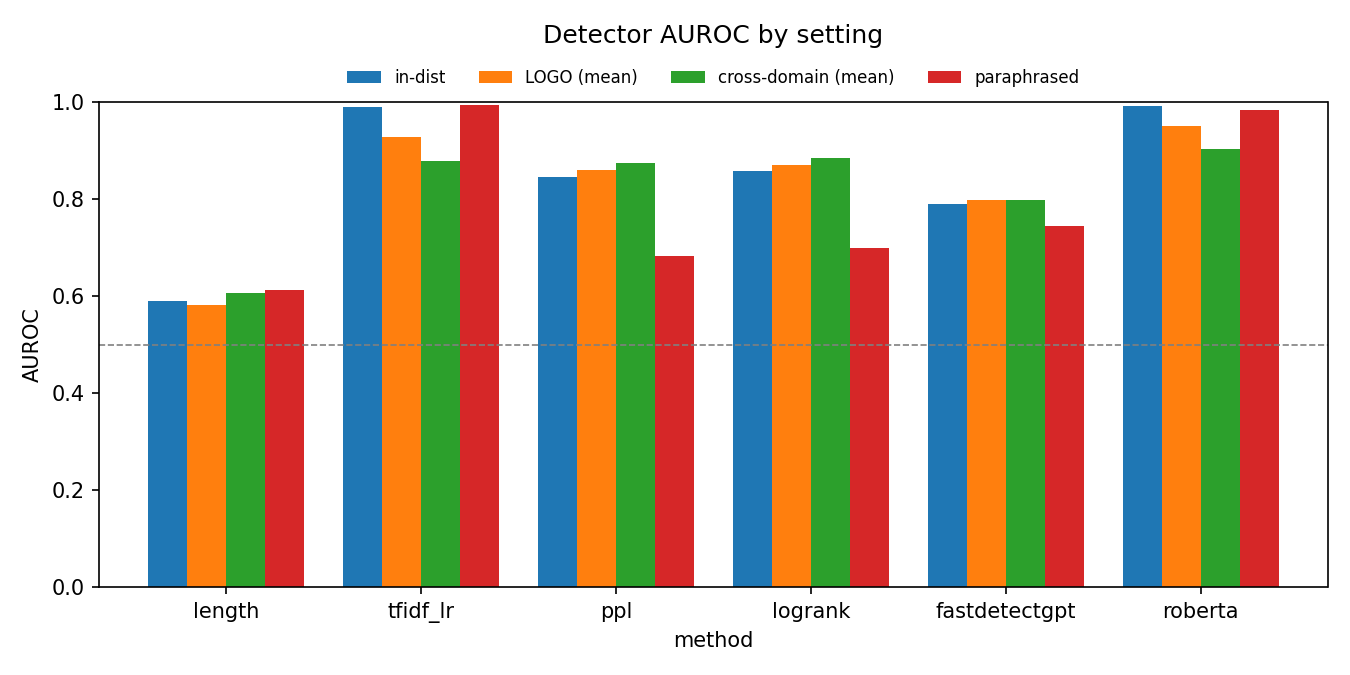
\includegraphics[width=\textwidth]{figures/fig1_auroc_by_setting.png}
%   \caption{AUROC of each detector by setting group.}
%   \label{fig:bars}
% \end{figure}
% \begin{figure}
%   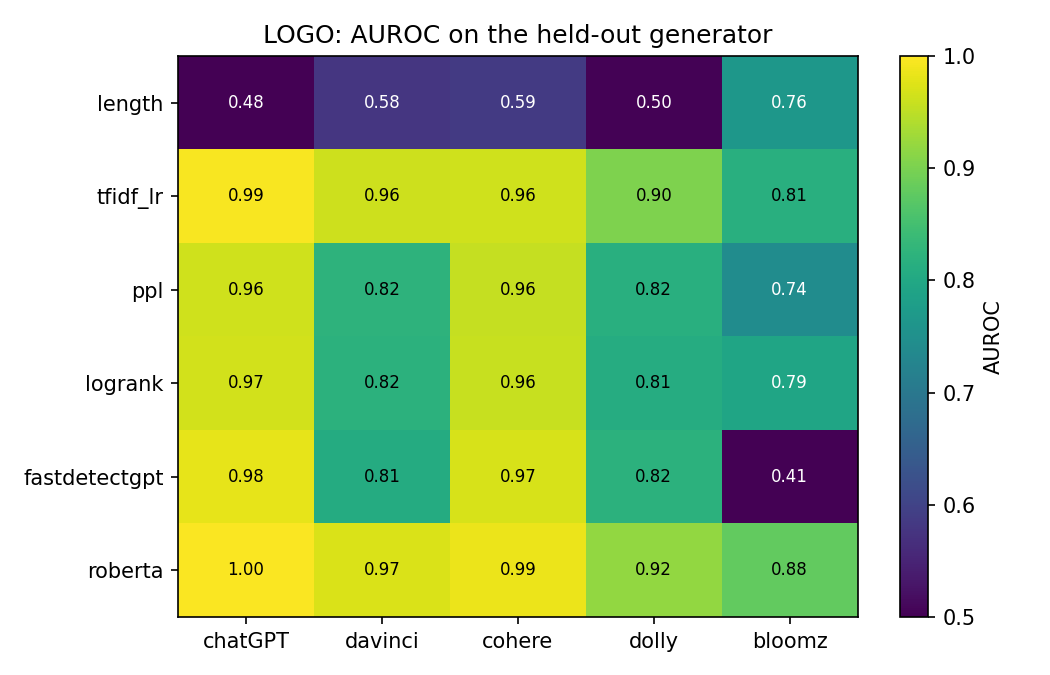
\includegraphics[width=0.8\textwidth]{figures/fig2_logo_heatmap.png}
%   \caption{Leave-one-generator-out AUROC.}
%   \label{fig:logo}
% \end{figure}

\section{Discussion}

\TBD{Write only what Tables~\ref{tab:indist}--\ref{tab:para} support. Questions to answer:
(1) how much each method drops from in-distribution to unseen generators and domains, and which generator and domain
are hardest; (2) whether zero-shot methods drop less than trained ones; (3) where the length-only model is clearly
above 0.5, which signals a length shortcut in that setting; (4) how much each method loses under the paraphrase attack,
and whether paraphrased human texts are flagged as machine (detecting paraphraser style rather than LLM authorship);
(5) what the top TF-IDF features in \texttt{results/tfidf\_lr/indist/top\_features.csv} suggest.}

\section{Limitations}

\begin{itemize}
  \item We ran Fast-DetectGPT, the single-pass analytic form of DetectGPT's probability curvature, instead of
        perturbation DetectGPT \cite{mitchell23}, which needs about 20 T5 rewrites and 21 scoring passes per text and
        did not fit our GPU budget. Fast-DetectGPT scores a 1,500-text subset, so its LOGO and cross-domain
        estimates rest on fewer texts and have wider intervals.
  \item One zero-shot scorer (GPT-2 medium, 256 tokens); none of the M4 generators is GPT-2, so these methods are
        black-box here, and a stronger scorer could change their ranking.
  \item RoBERTa is trained for one epoch with default hyperparameters and a 256-token limit. Its validation set is
        used both for checkpoint selection and for the threshold, so its accuracy and F1 are slightly optimistic
        (AUROC is not affected).
  \item English only, at most 1,000 machine texts per cell, one paraphraser, and one seed: the confidence
        intervals capture test-set sampling, not training variance.
\end{itemize}

\section{Conclusion}

\TBD{Two or three sentences, from the results only.}

\section*{Reproducibility}
All code, split files and results are in the team repository
(\texttt{github.com/NIRMAL20062/generated\_text\_detection}). Every run writes \texttt{run\_info.json} with the git
commit, seed, hyperparameters, hardware and runtime; the README lists every command, and each script has a
\texttt{--dev} mode that runs on a committed sample in under two minutes.

\section*{Author contributions}
N.\ Kumar: data pipeline, splits, shared evaluator, baselines, tables. V.\ Kumar: RoBERTa detector.
R.\ Jha: zero-shot detectors. V.\ Kumar: paraphrase attack and results. \TBD{Each member checks their line.}

\begin{thebibliography}{}
  \bibitem[\protect\citename{Bao {\it et al.}\ }2024]{bao24}
   Bao, G., Zhao, Y., Teng, Z., Yang, L. and Zhang, Y. (2024) Fast-DetectGPT: efficient zero-shot detection of
   machine-generated text via conditional probability curvature. In {\it International Conference on Learning
   Representations (ICLR)}. arXiv:2310.05130.
  \bibitem[\protect\citename{Liu {\it et al.}\ }2019]{liu19}
   Liu, Y., Ott, M., Goyal, N., Du, J., Joshi, M., Chen, D., Levy, O., Lewis, M., Zettlemoyer, L. and Stoyanov, V.
   (2019) RoBERTa: a robustly optimized BERT pretraining approach. arXiv:1907.11692.
  \bibitem[\protect\citename{Mitchell {\it et al.}\ }2023]{mitchell23}
   Mitchell, E., Lee, Y., Khazatsky, A., Manning, C. D. and Finn, C. (2023) DetectGPT: zero-shot machine-generated
   text detection using probability curvature. In {\it International Conference on Machine Learning (ICML)}.
   arXiv:2301.11305.
  \bibitem[\protect\citename{Wang {\it et al.}\ }2024]{wang24}
   Wang, Y., Mansurov, J., Ivanov, P., Su, J., Shelmanov, A., Tsvigun, A., Whitehouse, C., Mohammed Afzal, O.,
   Mahmoud, T., Sasaki, T., Arnold, T., Aji, A. F., Habash, N., Gurevych, I. and Nakov, P. (2024) M4:
   multi-generator, multi-domain, and multi-lingual black-box machine-generated text detection. In {\it Proceedings
   of EACL}. arXiv:2305.14902.
\end{thebibliography}

\label{lastpage}

\end{document}
